\subsubsection{\stid{1.07} Exascale MPI} \label{subsubsect:mpich}
\paragraph{Overview}

MPI has been the de facto standard programming model for HPC from the
mid 90's till today, a period where supercomputing performance
increased by six orders of magnitude.  The vast majority of DOE's
parallel scientific applications running on the largest HPC systems
use MPI. These application codes represent billions of dollars of
investment. Therefore, MPI must evolve to run as efficiently as
possible on Exascale systems. Our group at Argonne developed a
high-performance, production-quality MPI implementation, called MPICH.
The focus areas of the Exascale MPI / MPICH project are: (1)
continuous improvement of the performance and capabilities of the
MPICH software to meet the demands of ECP and other broader DOE
applications, (2) coordinate vendor and supercomputing center
interactions to ensure efficient solutions to applications, and (3) be
involved in the MPI forum and standardization efforts to ensure
continuity of the work beyond this project.

MPICH team is involved in the formation of the MPI Forum and have been
deeply involved in defining the MPI standard since 1992. MPICH has
helped prototype and define the majority of the features in the MPI
standard. As such, MPICH has been one of the most influential pieces of
software in accelerating the adoption of the MPI standard by the HPC
community. MPICH has been adopted by leading vendors into their own
derivative implementations. Examples include Intel (for Intel MPI), Cray
(for Cray MPI), IBM (for IBM PE MPI), Mellanox (for MLNX-MPI), Microsoft
(for MS-MPI), and Ohio State University (for MVAPICH). MPICH and its
derivatives are exclusively used in 7 of the top 10 supercomputers in
the world today. MPICH is the recipient of a number of awards including
an R\&D 100 award.

\paragraph{Key Challenges}

While we believe MPI is a viable programming model at Exascale, both
the MPI standard and MPI implementations have to address the
challenges posed by the increased scale, performance characteristics
and evolving architectural features expected in Exascale systems, as
well as the capabilities and requirements of applications targeted at
these systems. The key challenges are:

\begin{enumerate}

\item Interoperability with intranode programming models having a high
  thread count~\cite{Hybrid1, Hybrid2, FT2} (such as OpenMP,
  OpenACC and emerging asynchronous task models);

\item Scalability and performance over complex
  architectures~\cite{Perf1, Perf2, FT2, Perf4} (including high core
  counts, processor heterogeneity and heterogeneous memory);

\item Software overheads that are exacerbated by lightweight cores and
  low-latency networks;

\item Enhanced functionality (extensions to the MPI standard) based on
  experience with applications and high-level libraries/frameworks
  targeted at Exascale; and

\item Topics that become more significant as we move to the next
  generation of HPC architectures: memory usage, power, and
  resilience.

\end{enumerate}

\paragraph{Solution Strategy}

The Exascale MPI project has the following primary technical thrusts:
(1) \textbf{Performance and Scalability} (2) \textbf{Heterogeneity}
(3) \textbf{Topology Awareness} (4) \textbf{Fault Tolerance} and (5)
\textbf{MPI+X Hybrid Programming}.

Our solution strategy started by addressing performance and
scalability aspects in MPICH related to network address
management~\cite{memscal}.  Apart from this, we also looked at
communication strategies which allow the MPI library to be as
lightweight as possible~\cite{ch41, ch42}. Other solutions include
investigation and evaluation of communication relaxation hints,
investigation of optimizations to memory scalability in MPICH and
improvements to MPI RMA operations.

Exascale MPI heterogeneity efforts~\cite{Hetero1, Hetero2, Hetero3}
started with the survey on heterogeneous memory architectures on
upcoming DOE machines and how MPICH can take advantage of
them~\cite{hexe}. The efforts also included the investigation of
utilizing heterogeneous memory inside the MPI implementation and
evaluation of applications~\cite{hetero4}. The heterogeneity efforts
further extended to investigating and developing technologies for GPU
integration for the better support of the coming Exascale
supercomputers.

Exascale MPI topology awareness efforts~\cite{Topo1,Topo2} originated
with the investigation and evaluation of hints based on topology
awareness and optimizations to virtual topology functionality in
MPICH~\cite{topo-io,topo-io2}. The other efforts include investigation
of topology-aware collectives and neighborhood collectives in
MPICH~\cite{coll} and evaluation of the selected ECP applications.

Exascale MPI fault tolerance efforts~\cite{FT1, FT2} started with
support for handling noncatastrophic errors in MPI. The second effort
included defining the scope of errors in MPI, a prerequisite for
user-level failure mitigation. Other efforts in this direction
includes standardizing these efforts in MPI and evaluating application
suitability for fault tolerance.

Exascale MPI+X hybrid programming developed firstly with effort in
improving interoperation of MPICH with threads~\cite{interthread}.
Secondly, we developed the work-queue data transfer model for
multithreaded MPI communication~\cite{workq}. We have included support
for interaction of MPICH with user-level thread (ULT)
libraries~\cite{ULT}, primarily targeting Argobots and the BOLT
runtime~\cite{BOLT}.  Other issues that are being looked at include the
investigation and evaluation on multiple virtual communication
interfaces for multithreaded MPI communication~\cite{VCI}.

\paragraph{Recent Progress}

The recent release of MPICH 3.4b1 version includes deliverables from the
major milestones of FY2020. Figure~\ref{fig:fy20} provides the details
of them. In the first milestone, we created the collective algorithm
selection framework which allows MPI to choose different algorithm for
collectives operations based on multiple factors including number of
processes, network topology and support of hardware acceleration. The
user of MPICH can provide a configuration file to describe the criteria
for choosing different collective algorithms. We expect the vendors
utilizing this capability to provide collective selection strategies
that is optimized for the target supercomputers. The end-user could also
generate their own strategies that is fine-tuned to the characteristic
and needs of their applications.
In the second milestone, we added the support for GPU in MPI
communication. This allows a buffer in the GPU memory to be used
directly in MPI communication operations. MPICH's GPU support can
utilize the native support of fast GPU communication in hardware while also
provide a fallback mode for more complex MPI communication pattens. We
also created a new high-performance datatype engine that further
utilizes GPU for handling non-contiguous datatype in MPI communication.

Lastly, we made many efforts in participating the standardization of
MPI-4 by discussing proposed features and contributing the feedback for
our users back to the MPI forum. This has led to several new features
being accepted by the MPI Forum.

\begin{figure}[htb]
  \centering
  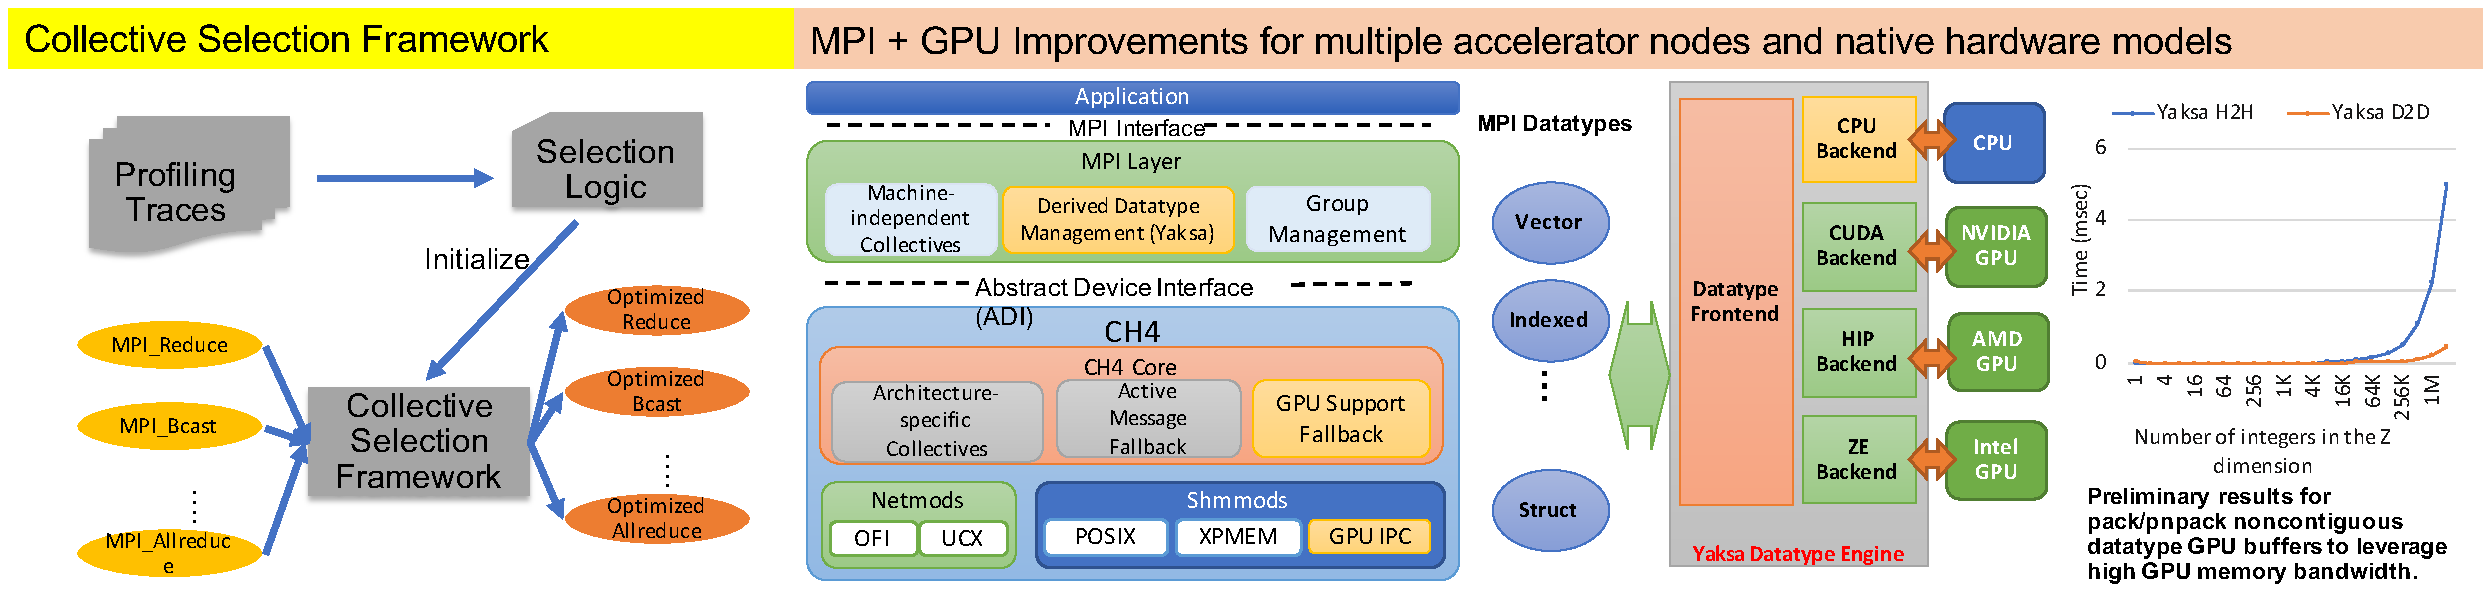
\includegraphics[width=6in]{projects/2.3.1-PMR/2.3.1.07-Exascale-MPI/MPICH-recent-milestones.pdf}
  \caption{\label{fig:fy20}Major MPICH milestones completed in fiscal year 2020}
\end{figure}

\paragraph{Next Steps}
A major focus of the ongoing Exascale MPI efforts is further
improvements to the MPI+GPU support. This includes support for GPU
stream triggered MPI operations, optimized support for noncontiguous
data and software evaluations. Another focus of FY2021 is the
implementation of new features in MPI-4 standard including persistent
collective operations. We will also make effort for improving the MPICH
testing infrastructure by improving the testsuite and promoting
integration ECP systems to provide better test coverage and a
close-to-production test environment. This would enhance the readiness
of MPICH for exascale systems.
